\begin{figure}[H]
    \centering
    \begin{subfigure}{0.32\textwidth}
        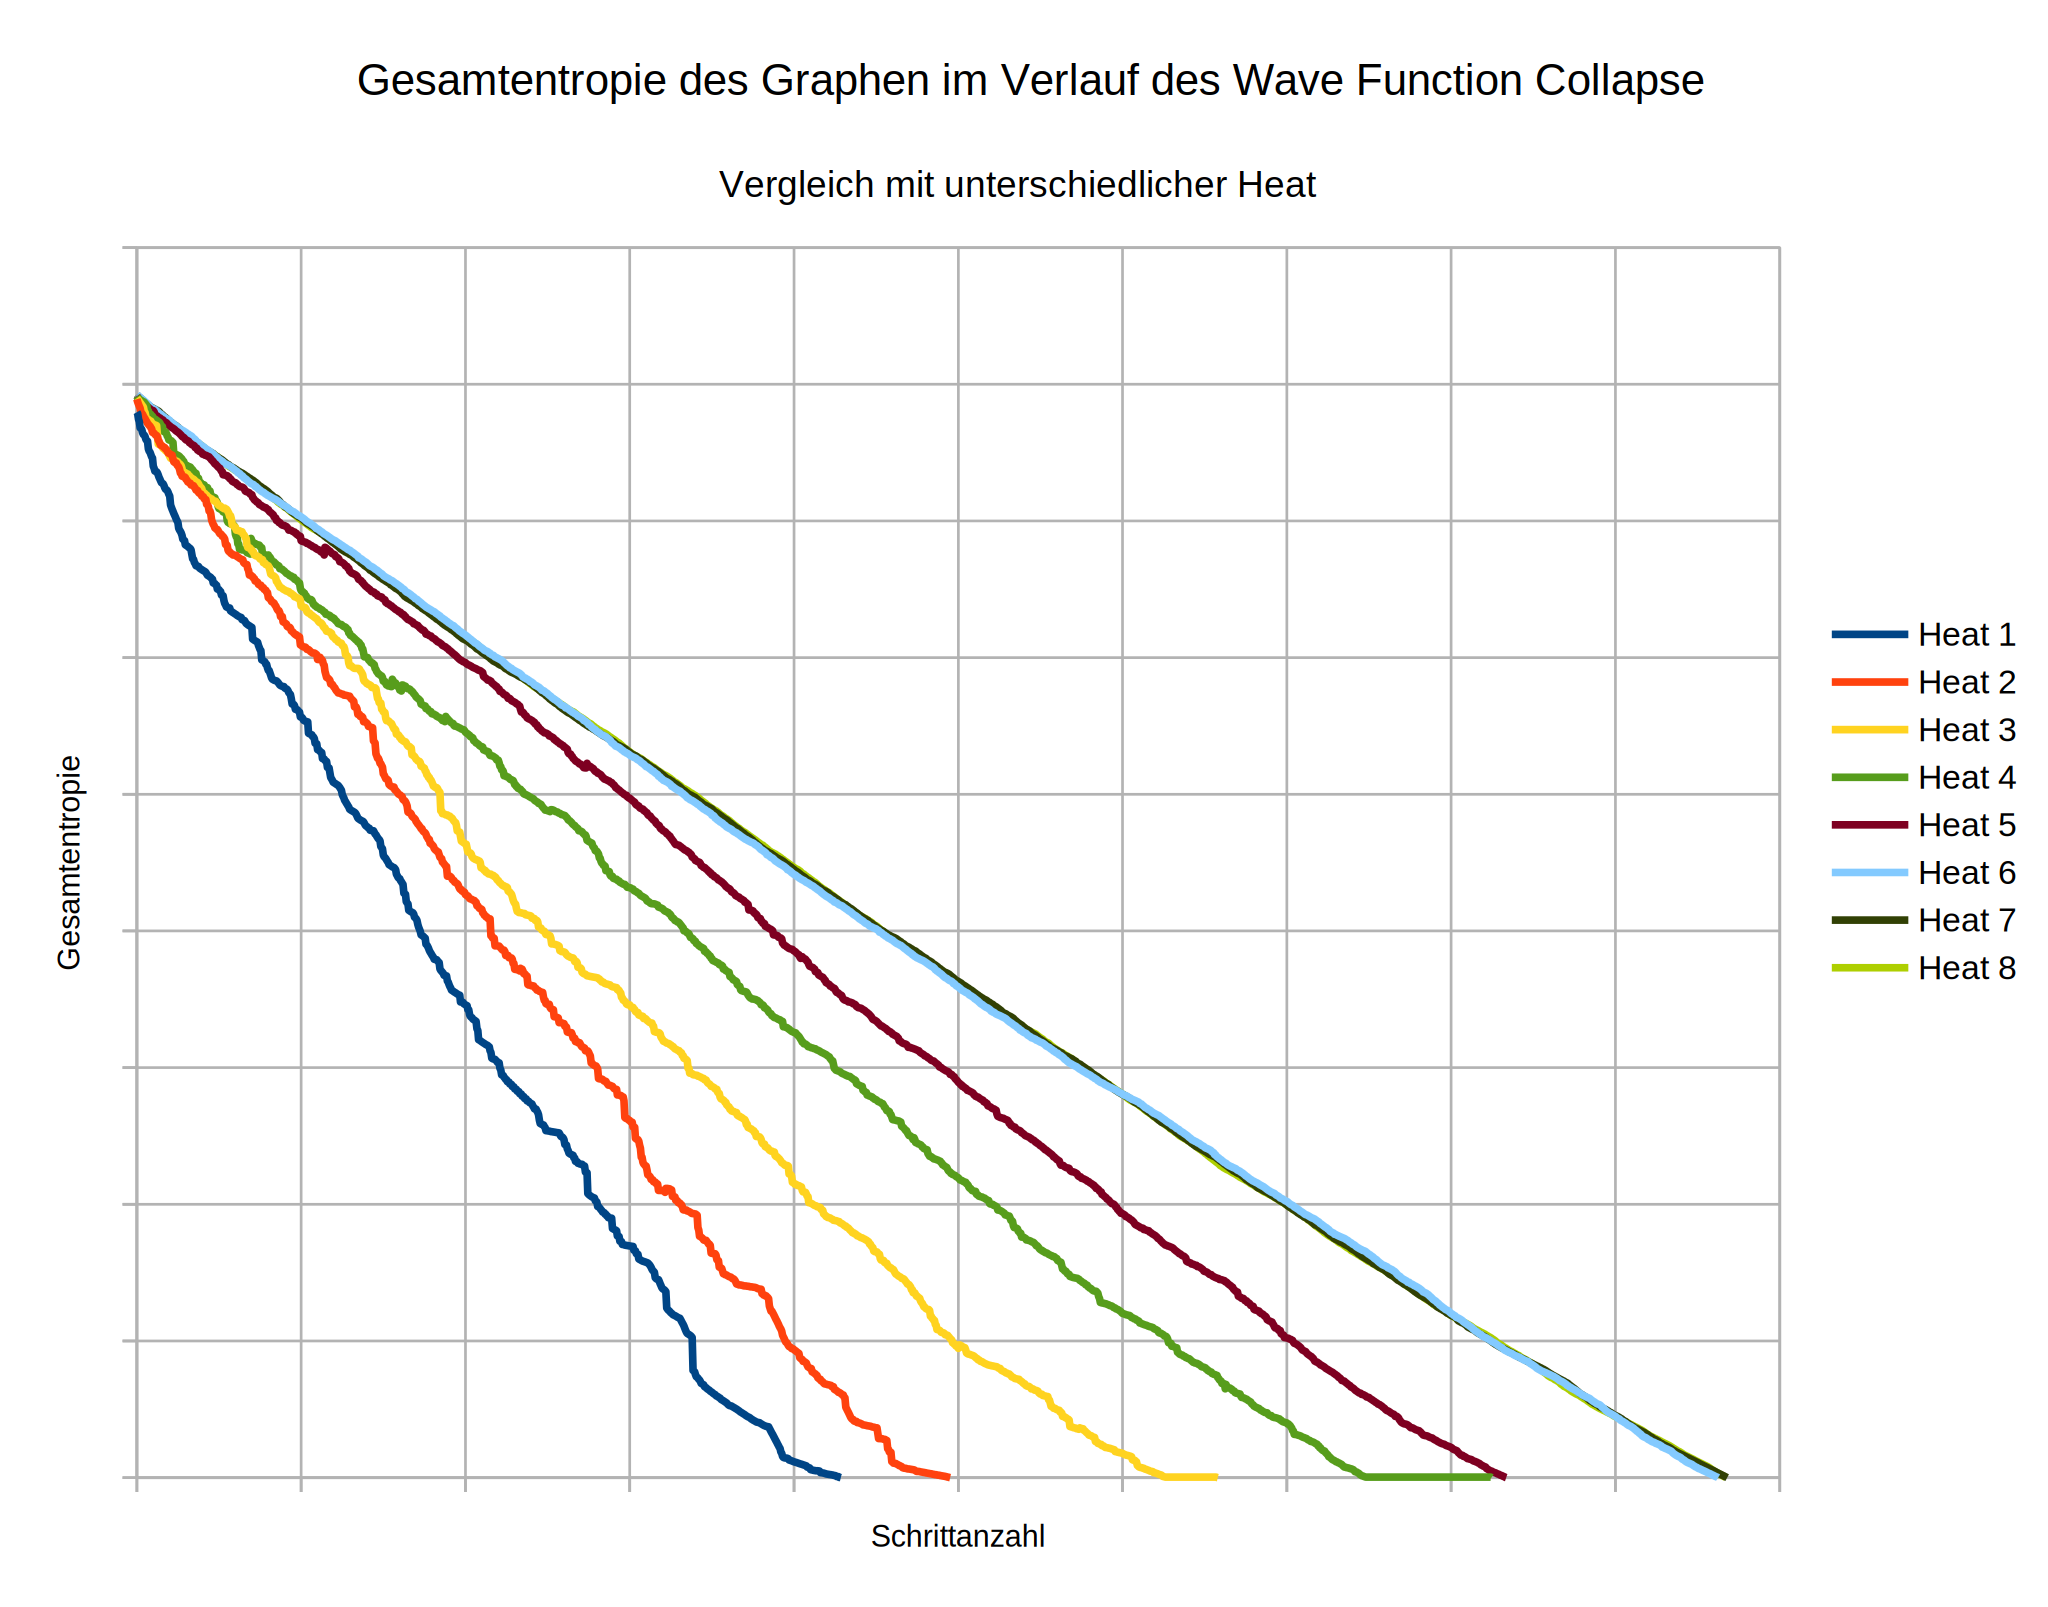
\includegraphics[width=\linewidth]{data/extract_wrapping/1.png} \caption{}
    \end{subfigure}
    \begin{subfigure}{0.32\textwidth}
        \includegraphics[width=\linewidth]{data/extract_wrapping/2.png} \caption{}
    \end{subfigure}
    \begin{subfigure}{0.32\textwidth}
        \includegraphics[width=\linewidth]{data/extract_wrapping/3.png} \caption{}
    \end{subfigure}
    
    \vspace{4mm}
    
    \begin{subfigure}{0.24\textwidth}
        \includegraphics[width=\linewidth]{data/extract_wrapping/4.png} \caption{}
    \end{subfigure}
    \begin{subfigure}{0.24\textwidth}
        \includegraphics[width=\linewidth]{data/extract_wrapping/5.png} \caption{}
    \end{subfigure}
    \begin{subfigure}{0.24\textwidth}
        \includegraphics[width=\linewidth]{data/extract_wrapping/6.png} \caption{}
    \end{subfigure}
    \begin{subfigure}{0.24\textwidth}
        \includegraphics[width=\linewidth]{data/extract_wrapping/7.png} \caption{}
    \end{subfigure}
    
    \caption{
        Extraktion mit vertikalem Wrapping. (a-c) zeigen wie einige Zustände über die Umfelder aus dem Beispiel extrahiert werden. (b) Umfeld $U_2$ und $U_3$ sind gleich, somit hat Zustand $Z_2$ eine Frequenz von 2. (c) $U_4$ überschreitet den Rand und nimmt die Pixel aus der ersten Reihe. (d-g) zeigt welche Zustände überlappen. (d) zeigt, dass $Z_1$ nördlich von $Z_2$ und umgekehrt $Z_2$ südlich von $Z_1$ platziert werden kann. (d-f) liegen einfach im Beispiel nebeneinander, während in (g) so nicht direkt im Beispiel vorkommt, aber dennoch eine valide Überlappung ergibt.
    }
    \label{fig:extract_wrapping}
\end{figure}